\section{Assessing Risk Preferences: A Dual-Criterion Approach}
\subsection{Setup and Definitions}
The results of section \ref{return_section} paint very different pictures of retail investors. 
Using the method set forth by \cite{Welch2022} and \cite{Fedyk2024}, analysed also in section \ref{fedyk_paper_returns}, yields superior returns and similar drawdowns to the market.
They also conclude that the Robinhood crowd has achieved positve alpha when analysed under different factor models (table VII, IX, X in \cite{Welch2022} and table 16 in \cite{Fedyk2024}). 
These results appear to be in contrast with the existing literature on the retail investing, most notably \cite{BarberOdean2000}.

A more fundamental question, however, is whether those returns are attractive once investors' attitudes toward risk are taken into account.
This section evaluates the Robinhood portfolio against its market benchmarks using two complementary criteria.

First, I adopt the constant-relative-risk-aversion (CRRA) framework, in line with the majority of asset pricing work.
\begin{equation}
    U(W) = 
    \begin{cases}
    \frac{W^{1-\gamma}-1}{1-\gamma}, \gamma\neq 1\\
    \ln(W), \gamma = 1
    \end{cases}
    \label{CRRA}
\end{equation}

By computing expected utility of both the Robinhood and benchmark portfolios over a grid of possible risk aversion ($\gamma$) values,
I identify the cutoff $\gamma^*$ such that a representative CRRA investor is indifferent between the two.
This delivers a concise, parametric summary of how risk preferences may shape portfolio choice.

However, this method cannot deliver precise estimates given the limited sample size. 
I therefore employ another method to directly estimate the risk aversion $\gamma$, 
following the Generalized Method of Moments (GMM) framework introduced by \cite{hansen1982generalized} to find the risk aversion that satisfies the intertemporal Euler Condition.

\begin{equation}
    \mathbb{E}\left[ \beta \frac{U^\prime(c_{t+1})}{U^\prime(c_{t})}R_{t+1} \right] = 1
    \label{euler_def}
\end{equation}  
where $R_{t+1}$ is the realized gross return on the asset at time $t+1$.

Rewriting equation \ref{euler_def} and assuming CRRA utility we arrive at the following condition:
\begin{equation}
    \mathbb{E}\left[ \beta \left( \frac{c_{t+1}}{c_{t}} \right)^{-\gamma} R_{t+1} \right] = 1
\end{equation}  

Then, using portfolio returns as a proxy of consumption and letting $\beta = \frac{1}{1+\bar{r_f}}$ we derive the following GMM moment condition:
\begin{equation}
    g(\gamma) = \mathbb{E} \left[ \frac{R_{t+1}^{-\gamma}}{1+\bar{r}_f}  R_{t+1} - 1\right] = 0
    \label{gmm_condition}
\end{equation}  

I then use a root-solving algorithm to find the $\gamma$ that satisfies equation \ref{gmm_condition}. 



Second, I apply first- and second-order stochastic dominance tests (FSD and SSD) to the same return distributions.
This allows to avoid unnecesary, though conventional, assumptions regarding functional forms or parameterisation.
Log-Normality might well not be respected for different distributions, stochastic dominance tests take into account the shape of empirical CDFs to answer stronger questions. 

\subsection{Expected Utility and Cutoff}
As birefly explained above, finding a cutoff value for risk aversion delivers a concise summary for what paramaters of risk aversion a rational utility-maximizer agent with CRRA utility would choose the Robinhood portfolio,
the limited size and noise of the sample imply wide conference intervals for the estimated expected utilities.
In practice, this remains a useful conceptual framework to understand how risk preference and believes may affect portfolio choice, but in limited samples its numerical outputs are more illustrative than definitive.
However, this method yields precise results in a very specific case I will describe later. 

Formally, we want to find $\gamma^*$ defined as:
\begin{equation}
    \gamma^* = \min\left\{ \gamma_j : \mathbb{E}[U_p(\gamma_j)] \geq \mathbb{E}[U_m(\gamma_j)] \right\}
    \label{gamma_cutoff}
\end{equation}
where $U_p(\cdot)$ is the utility of the Robinhood portfolio, while $U_m(\cdot)$ is the utility of the market portfolio.

In practice, this methods applies the CRRA utility function (\ref{CRRA}) to each gross return observation and then takes the sample average,
effectively taking the resulting mean as the investor's expected utility at the final date based on the history of realized returns.
Gross returns are the equal to the wealth at time $t$, assuming the initial wealth $W$ to be equal to one without loss of generality.

The main problem related to this approach is inherent to the sample we apply it to, having only 539 observations and inclusion of extreme events such as the COVID crash. 
These factors inflate the sample variability of our mean-utility estimates, so much that regardless of whether we use daily returns, various rolling-window horizons, or subperiods, the resulting confidence intervals remain prohibitively wide.
Figure \ref{fig:cutoff} illustrates this well: 
\begin{figure}[h!]
    \centering
    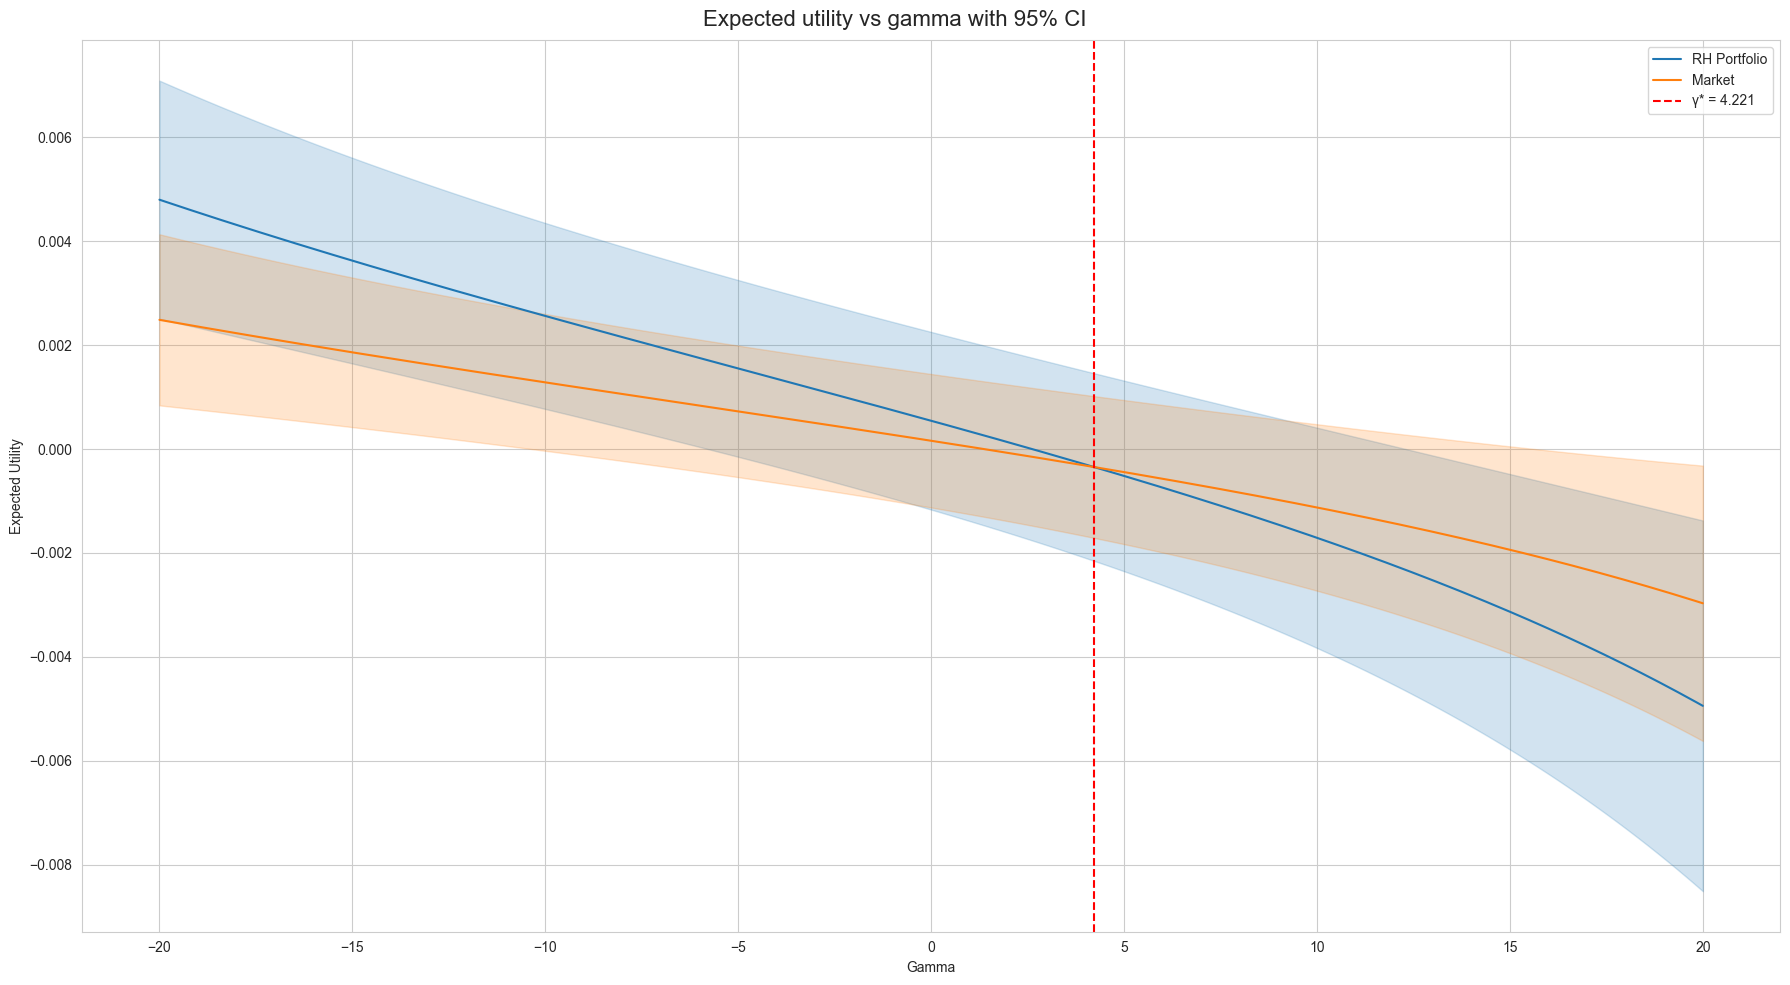
\includegraphics[width=\linewidth]{../images/risk/cutoff_daily.png}
    \caption{Utility for the Robinhood and Market portfolios evaluated over a grid of $\gamma$.}
    \label{fig:cutoff}
\end{figure}

\subsection{Augmented Return Sample via All Date-Pairs}

To overcome the limited information in only 539 daily observations, we construct an "all-pairs" dataset that dramatically amplifies our effective sample.  
Specifically, let the trading-day indices in our original series be $1,2,\dots,T$.  
For every ordered pair of dates $(i,j)$ with $1 \le i < j \le T$, we compute the cumulative excess return (net of the risk-free rate) between day $i$ and day $j$ as
\begin{equation}
    R_{i,j}
    \;=\;
    \prod_{k=i+1}^{j}\bigl(1 + r_k - r_{f,k}\bigr),
    \quad
    1 \le i < j \le T,
    \label{eq:allpairs_return}
\end{equation}
where $r_k$ is the gross portfolio return on day $k$ and $r_{f,k}$ is the daily risk-free rate.  
We treat each multi-day return $R_{i,j}$ as a separate outcome in the investor's distribution of possible holding-period returns, we increase the number of observations from $T$ to $T(T-1)/2$, which reduces sampling variability in our utility-based estimates.  
This "all-pairs" approach preserves the time-ordering of returns while allowing us to evaluate expected-utility cutoffs with far greater precision.  

In practice, this results in finding a very low $\gamma^*$ that satisfies equation \ref{gamma_cutoff}, meaning that every investor with a reasonable risk-aversion parameter under CRRA utility would have a greater utility by investing in the market.
In some case, particularly when ending the sample before the pandemic, the utility curves fitted on the "all-pairs" dataset simply do not intersect for a wide grid of possible risk aversion,
and in fact we find also that in these cases the market stochastically dominates the robinhood portfolio (something which will be analysed more in depth later).

Detailed cutoff plots are shown above for the whole period.
WHY IS THE MARKET different!!!!!!!!

\begin{figure}[h!]
  \centering
  \subfloat[Number of all-pairs returns]{%
    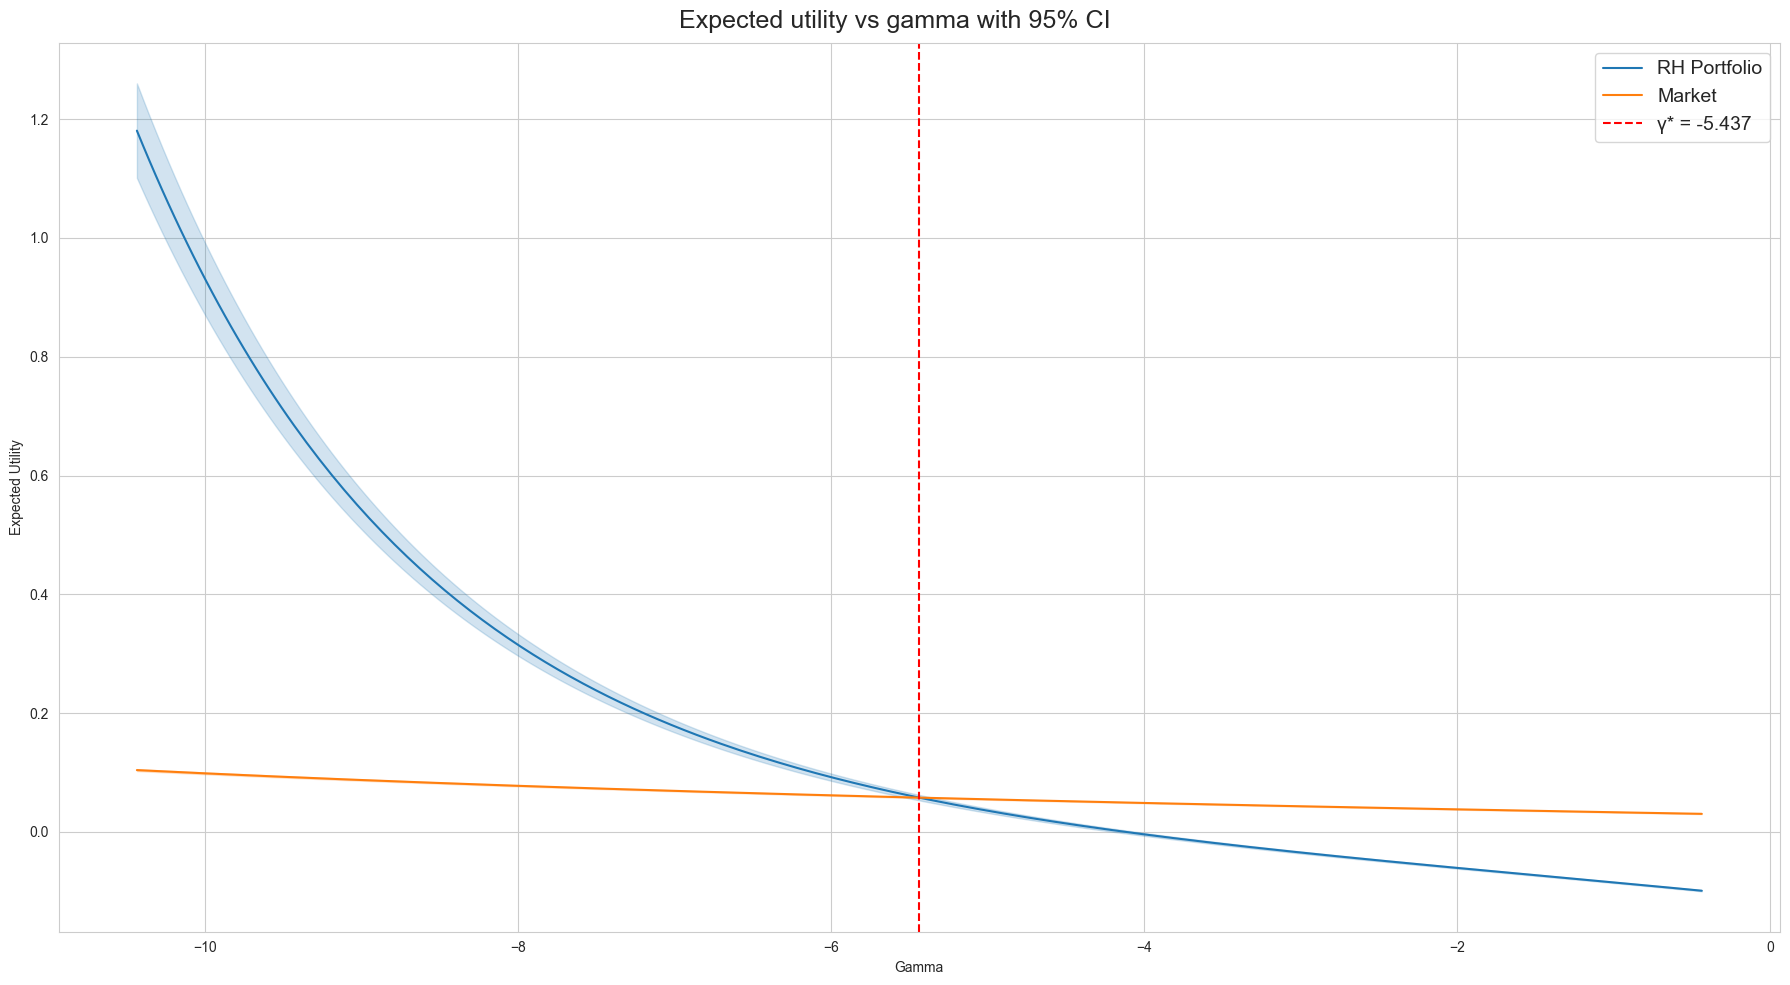
\includegraphics[width=0.48\textwidth]{../images/risk/cutoff_number_all.png}%
    \label{fig:cutoff_number_all}
  }
  \hfill
  \subfloat[Wealth evolution for each return]{%
    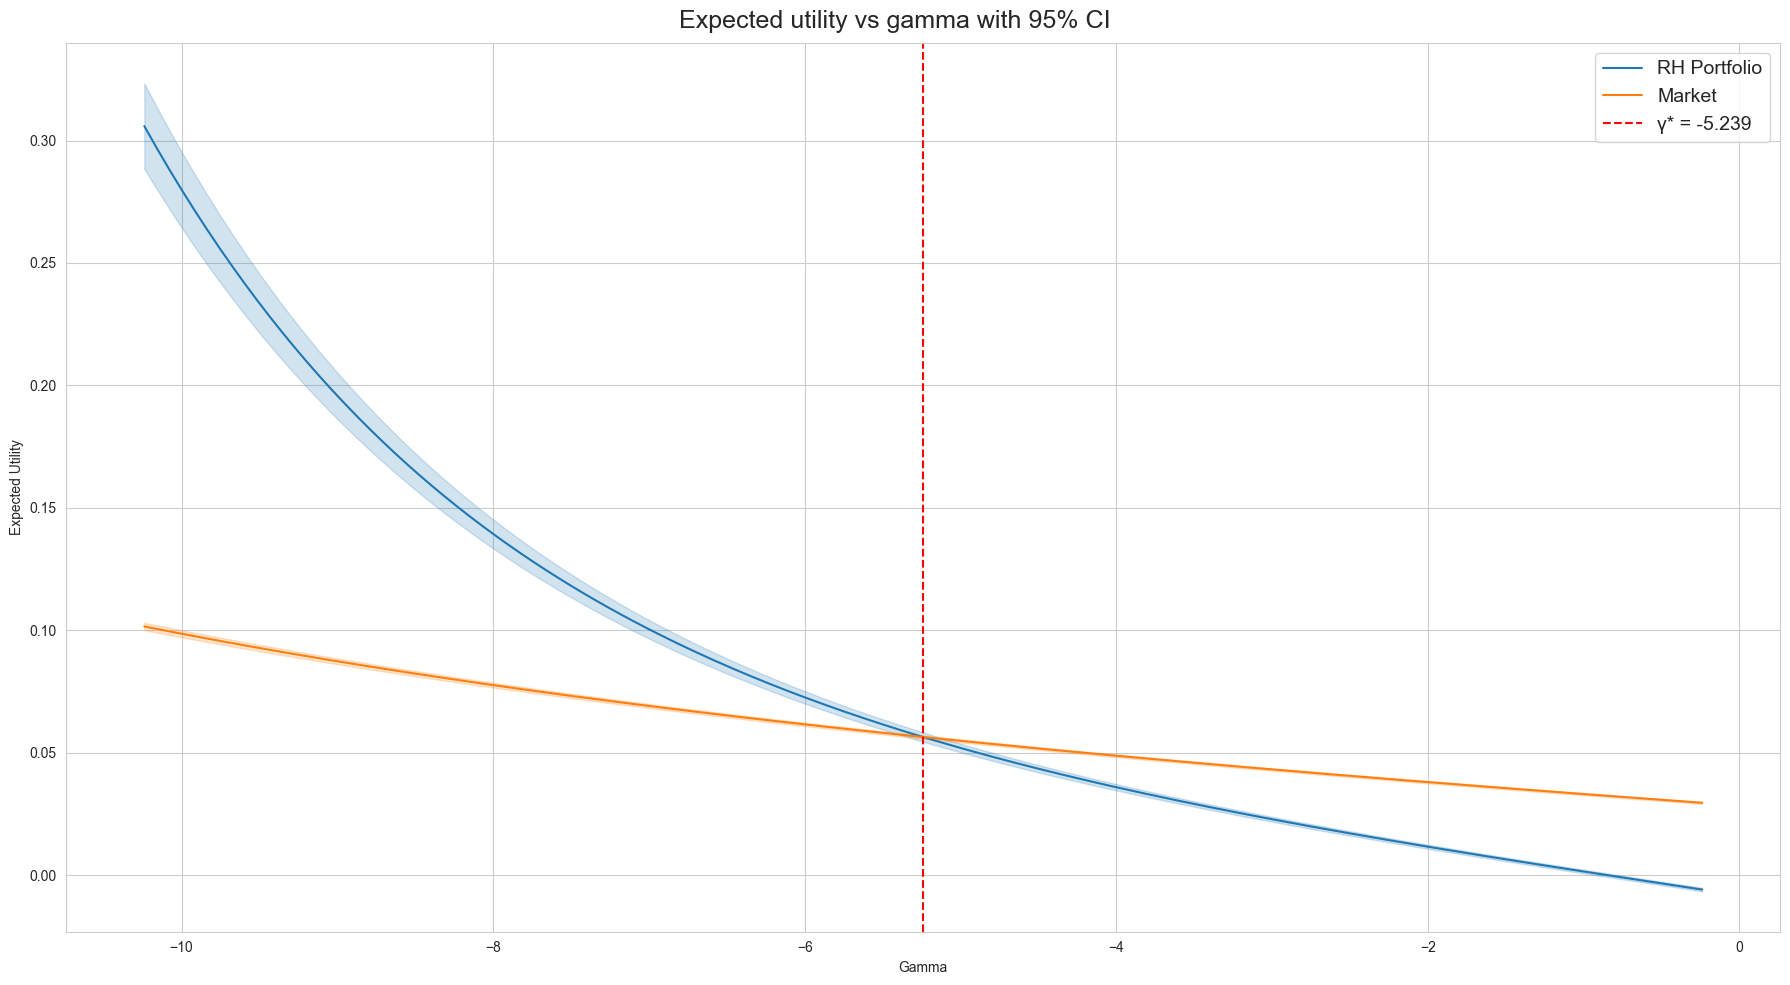
\includegraphics[width=0.48\textwidth]{../images/risk/cutoff_wealth_all.png}%
    \label{fig:cutoff_wealth_all}
  }
  \caption{(a) Total number of paired returns computed; (b) Corresponding compounded wealth paths.}
  \label{fig:cutoff_all_sidebyside}
\end{figure}
